\documentclass[11pt]{article}
\usepackage{amsmath,amsbsy,amssymb,verbatim,fullpage,ifthen,graphicx,bm,amsfonts,amsthm,url}
\usepackage{graphicx}
\usepackage{xcolor}
%\usepackage[dvipsnames]{xcolor}
\usepackage{algpseudocode}
\newcommand{\mfile}[1]  {{\small \verbatiminput{./#1}}} % Jeff Fessler, input matlab file
\newcommand{\tmop}[1]{\ensuremath{\operatorname{#1}}}
\newcommand{\R}{\mathbb{R}}
\newcommand{\C}{\mathbb{C}}
\newcommand{\Z}{\mathbb{Z}}
\newcommand{\A}{\mathcal{A}}
\newcommand{\minimize}{\operatorname*{minimize\ }}
\newcommand{\maximize}{\operatorname*{maximize}}
\newcommand{\opdet}[1]{\operatorname{\textbf{det}}\left(#1\right)}
\newcommand{\optr}[1]{\operatorname{\textbf{tr}}\left(#1\right)}
\newcommand{\answer}[2][blue]{\ifdefined\AnswerDefine{\color{#1}\it#2}\fi}
\newcommand{\mtx}[1]{\mathbf{#1}}
\newcommand{\vct}[1]{\mathbf{#1}}
\def \lg       {\langle}
\def \rg       {\rangle}
\def \mA {\mtx{A}}
\def \mB {\mtx{B}}
\def \mI {\mtx{I}}
\def \mJ {\mtx{J}}
\def \mU {\mtx{U}}
\def \mS {\mtx{S}}
\def \mV {\mtx{V}}
\def \mW {\mtx{W}}
\def \mLambda {\mtx{\Lambda}}
\def \mSigma {\mtx{\Sigma}}
\def \mX {\mtx{X}}
\def \mY {\mtx{Y}}
\def \mZ {\mtx{Z}}
\def \zero     {\mathbf{0}}
\def \vzero    {\vct{0}}
\def \vone    {\vct{1}}
\def \vu {\vct{u}}
\def \vv {\vct{v}}
\def \vx {\vct{x}}
\def \vy {\vct{y}}
\def \vz {\vct{z}}
\def \vphi {\vct{\phi}}
\def \vmu {\vct{\mu}}
\def \R {\mathbb{R}}


\usepackage{xspace}
\makeatletter
\DeclareRobustCommand\onedot{\futurelet\@let@token\@onedot}
\def\@onedot{\ifx\@let@token.\else.\null\fi\xspace}

\def\eg{\emph{e.g}\onedot} \def\Eg{\emph{E.g}\onedot}
\def\ie{\emph{i.e}\onedot} \def\Ie{\emph{I.e}\onedot}
\def\cf{\emph{c.f}\onedot} \def\Cf{\emph{C.f}\onedot}
\def\etc{\emph{etc}\onedot} \def\vs{\emph{vs}\onedot}
\def\wrt{w.r.t\onedot} \def\dof{d.o.f\onedot}
\def\etal{\emph{et al}\onedot} \def\st{\emph{s.t}\onedot}
\pagestyle{plain}

\title{{\bf Homework Set 2, CPSC 8420, Fall 2023}} % Change to the appropriate homework number
\author{\Large\underline{Your Name}}
\date{\textbf{\Large\textcolor{red}{Due 10/26/2023, Thursday, 11:59PM EST}}} % put your name in the LastName, FirstName format
%\date{\today}

\begin{document}
	\maketitle
	

	\section{Problem 1}
	For PCA, from the perspective of maximizing variance, please show that the solution of $\bm{\phi}$ to $\maximize \|\mX \bm{\phi}\|^2_2, \st \ \|\bm{\phi}\|_2=1$ is exactly the first column of $\mU$, where $[\mU,\mS]=svd(\mX^T\mX)$. (Note: you need prove why it is optimal than any other reasonable combinations of $\mU_i$, say $\hat{\bm{\phi}}=0.8*\mU(:,1)+0.6*\mU(:,2)$ which also  satisfies $\|\hat{\bm{\phi}}\|_2=1$.)
	


	
	\vspace{4cm}
	\section{Problem 2}
	Given matrix $\mX\in\R^{n\times p}$ (assume each column is centered already), where $n$ denotes sample size while $p$ feature size. To conduct PCA, we need find eigenvectors to the  largest eigenvalues of $\mX^T\mX$, where usually the complexity is $\mathcal{O}(p^3)$. Apparently when $n\ll p$, this is not economic when $p$ is large. Please consider conducting PCA based on $\mX\mX^T$ and obtain the eigenvectors for $\mX^T\mX$ accordingly and use experiment to demonstrate the acceleration.
	\vspace{0.5cm}
	
	\subsection{eVec}
	Assume $\vv$ is an eigenvector of $\mX\mX^T$ to eigenvalue $\lambda$. Then is holds $$\mX\mX^T\vv=\lambda\vv$$ and 
	$$\mX^T\mX\mX^T\vv=\mX^T\lambda\vv =\lambda\mX^T\vv$$, hence $\mX^T\vv$ is an eignevector of $\mX^T\mX$  with eigenvalue $\lambda$

	\subsection{Exp}
	\mfile{q2.m}
	err =

   1.0e-14 *

    0.9770    0.1713    0.1028

	
	\section{Problem 3}
	Let's revisit Least Squares Problem: $\minimize \limits_{\bm{\beta}} \frac{1}{2}\|\vy-\mA\bm{\beta}\|^2_2$, where $\mA\in\R^{n\times p}$.
	\begin{enumerate}
		\item Please show that if $p>n$, then vanilla solution $(\mA^T\mA)^{-1}\mA^T\vy$ is not applicable any more.	
		\item Let's assume $\mA=[1, 2, 4;1, 3, 5; 1, 7, 7; 1, 8, 9], \vy=[1;2;3;4]$. Please show via experiment results that Gradient Descent method will obtain the optimal solution with  Linear Convergence rate if the learning rate is fixed to be $\frac{1}{\sigma_{max}(\mA^T\mA)}$, and $\bm{\beta}_0=[0;0;0]$.	
		\item Now let's consider ridge regression: $\minimize \limits_{\bm{\beta}} \frac{1}{2}\|\vy-\mA\bm{\beta}\|^2_2+\frac{\lambda}{2} \|\bm{\beta}\|^2_2$, where  $\mA,\vy,\bm{\beta}_0$ remains the same as above while learning rate is fixed to be $\frac{1}{\lambda+\sigma_{max}(\mA^T\mA)}$ where $\lambda$ varies from $0.1,1,10,100,200$, please show that Gradient Descent method with larger $\lambda$ converges faster. 
	\end{enumerate}

	\begin{enumerate}
		\item $\mA^T\mA$ is a $p\times p$ matrix, but the $rank(\mA^T\mA)\leq min(n,p) < n \implies \mA^T\mA$ is not invertable
		\item See figure \ref{fig:Q3_2} 
		\mfile{q3_2.m} 
		\begin{figure}[h!]
			\centering
			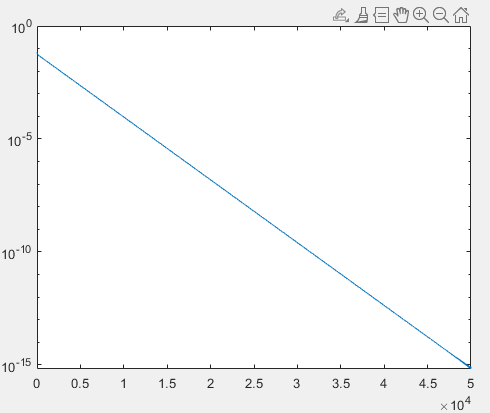
\includegraphics[width=0.5\linewidth]{q32.png}
			\caption{Q3-2}
			\label{fig:Q3_2}
		\end{figure}:

		\item See figure \ref{fig:Q3_3} 
		\mfile{q3_3.m} 
		\begin{figure}[h!]
			\centering
			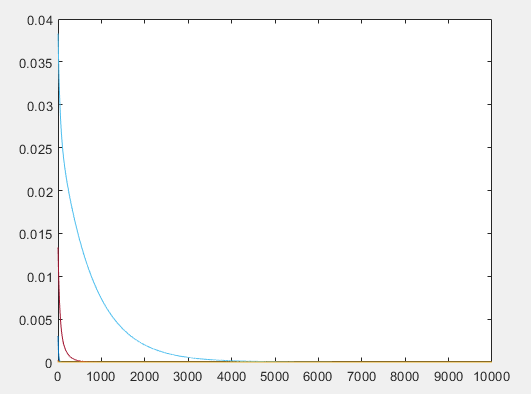
\includegraphics[width=0.5\linewidth]{q3_3.png}
			\caption{Q3-2}
			\label{fig:Q3_3}
		\end{figure}:
	\end{enumerate}
	
	\section{Problem 4}
	We consider matrix completion problem. As we discussed in class, the main issue of \textit{softImpute (Matrix Completion via Iterative Soft-Thresholded SVD)} is 
	when the matrix size is large, conducting \textit{SVD} is computational demanding. Let's recall the original problem where 
	$\mX, \mZ \in\mathbb{R}^{n\times d}$: 
	\begin{equation}\label{eq:nuc}
	\min\limits_{\mZ}\frac{1}{2}\|P_\Omega(\mX)-P_\Omega(\mZ)\|_F^2+\lambda \|\mZ\|_*
	\end{equation} 
People have found that instead of finding optimal $\mZ$, it might be better to make use of \textit{Burer-Monteiro} method to optimize two matrices $\mA \in\mathbb{R}^{n\times r}, \mB\in\mathbb{R}^{d\times r} (r\ge rank(\mZ^*))$ such that $\mA\mB^T=\mZ$. The new objective is:
	\begin{equation}\label{eq:bur}
	\min\limits_{\mA,\mB}\frac{1}{2}\|P_\Omega(\mX-\mA\mB^T)\|_F^2+\frac{\lambda}{2}(\|\mA\|_F^2+\|\mB\|^2_F).
\end{equation} 
\begin{itemize}
	\item Assume $[\mU,\mSigma,\mV]=svd(\mZ)$, show that if $\mA=\mU\mSigma^\frac{1}{2}, \mB=\mV\mSigma^\frac{1}{2}$, then Eq. (\ref{eq:bur}) is equivalent to Eq. (\ref{eq:nuc}).
	\item The \textit{Burer-Monteiro} method suggests if we can find  $\mA^*,\mB^*$, then the optimal $\mZ$ to Eq. (\ref{eq:nuc}) can be recovered by $\mA^*{\mB^*}^T$. It boils down to solve Eq. (\ref{eq:bur}). Show that we can make use of \text{least squares} with ridge regression to update $\mA, \mB$ row by row in an alternating minimization manner as below. Assume $n=d=2000, r=200$, please write program to find $\mZ^*$.
\end{itemize}
\begin{algorithmic}
	\State $T \gets 100, i\gets 1$ \ \% \textcolor{blue}{you can also set T to be other number instead of 100}
	\If{$i\leq T$} 
	\State $update \ A \ row \ by \ row \ while \ fixing \ B$
	\State $update \ B \ row \ by \ row \ while \ fixing \ A$
	\State $i \gets i+1$
	%\EndIf
	\EndIf 
\end{algorithmic}

\subsection{}
It is easy to prove that the parts in front of the plus sign in the two objects are equal  
\begin{equation}\label{eq:right}
	\frac{1}{2}\|P_\Omega(\mX)-P_\Omega(\mZ)\|_F^2 = \frac{1}{2}\|P_\Omega(\mX-\mA\mB^T)\|_F^2
\end{equation}
since $P_\Omega(\mX)-P_\Omega(\mZ) = P_\Omega(\mX-\mZ) =P_\Omega(\mX-\mA\mB^T)$.\\
For the part behind the addion sign, since
\begin{align*}
	\|\mA\|_F^2 &= \|\mU\mSigma^\frac{1}{2}\|_F^2 = trace(\mSigma^\frac{1}{2}\mU^T\mU\mSigma^\frac{1}{2}) = trace(\mSigma)\\
	\|\mB\|_F^2 &= \|\mV\mSigma^\frac{1}{2}\|_F^2 = trace(\mSigma^\frac{1}{2}\mV^T\mV\mSigma^\frac{1}{2}) = trace(\mSigma)\\
	\|\mZ\|_* &= trace(\mSigma)
\end{align*},
we can get \
\begin{equation}\label{eq:left}
	\frac{\lambda}{2}(\|\mA\|_F^2+\|\mB\|^2_F) = \lambda\|\mZ\|_*
\end{equation}
From (\ref{eq:right}) and (\ref{eq:left}), we can tell (\ref{eq:nuc}) is equivalent to (\ref{eq:bur})
\subsection{}
see figure \ref{fig:Q4_2}
\mfile{q4_2.m} 
		\begin{figure}[h!]
			\centering
			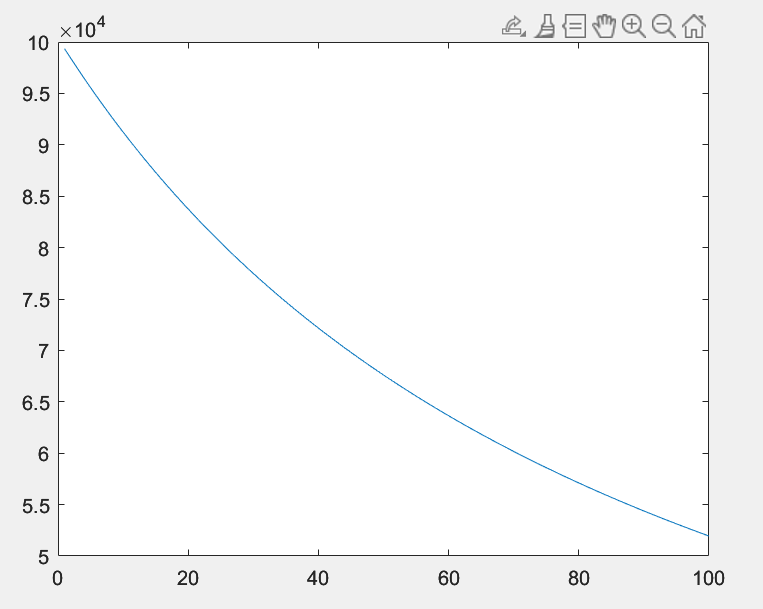
\includegraphics[width=0.5\linewidth]{q4_2.png}
			\caption{Q4-2}
			\label{fig:Q4_2}
		\end{figure}:
\end{document}
